%% ****** Start of file apsguide4-1.tex ****** %
%%
%%   This file is part of the APS files in the REVTeX 4.1 distribution.
%%   Version 4.1r of REVTeX, August 2010.
%%
%%   Copyright (c) 2009, 2010 The American Physical Society.
%%
%%   See the REVTeX 4.1 README file for restrictions and more information.
%%
\documentclass[preprint,secnumarabic,amssymb, nobibnotes, aip, prd]{revtex4-1}
%\usepackage{acrofont}%NOTE: Comment out this line for the release version!
\newcommand{\revtex}{REV\TeX\ }
\newcommand{\classoption}[1]{\texttt{#1}}
\newcommand{\macro}[1]{\texttt{\textbackslash#1}}
\newcommand{\m}[1]{\macro{#1}}
\newcommand{\env}[1]{\texttt{#1}}
\setlength{\textheight}{9.5in}


\usepackage{amsmath,amsfonts,amssymb}
\usepackage{graphicx}
\usepackage[colorlinks=true, allcolors=blue]{hyperref}


\usepackage{color}
\usepackage[latin9]{inputenc}
\usepackage{mathrsfs,amsmath}
\usepackage{graphicx}%
\usepackage{float}
\usepackage{amsfonts}%
\usepackage[titletoc]{appendix}
\usepackage{amssymb}
\usepackage{braket}
\usepackage{bm}

\newcommand{\mb}[1]{\bm{#1}}
\usepackage[T1]{fontenc}

\def\Nabla{\bm{\nabla}}
\def\bm{\mathbf}
\def\curl{\Nabla\times}
\def\div{\Nabla\cdot}
\def\lap{\Delta}
\def\vlap{\Delta}
\def\x{\hat{e}_{x}}
\def\y{\hat{e}_{y}}
\def\z{\hat{e}_{z}}
\def\p{\partial}
\def\h{\hat}
\def\h{\hat}
\def\tw{\tilde{\omega}}
\def\gm{\gamma}
\def\om{\omega}
\def\OM{\Omega}
\def\GM{\Gamma}
\def\dw{\delta\omega}
\def\dth{\Delta\theta}
\def\dk{\delta k}
\def\Hdth{\frac{\dth}{2}} %half Delta Theta
\def\P{\hat{\pi}_+}
\def\M{\hat{\pi}_-}


\DeclareMathOperator{\sech}{sech}
\DeclareMathOperator{\csch}{csch}
\DeclareMathOperator{\arcsec}{arcsec}
\DeclareMathOperator{\arccot}{arcCot}
\DeclareMathOperator{\arccsc}{arcCsc}
\DeclareMathOperator{\arccosh}{arcCosh}
\DeclareMathOperator{\arcsinh}{arcsinh}
\DeclareMathOperator{\arctanh}{arctanh}
\DeclareMathOperator{\arcsech}{arcsech}
\DeclareMathOperator{\arccsch}{arcCsch}
\DeclareMathOperator{\arccoth}{arcCoth} 

%\usepackage[font=small]{caption}
\newcommand{\includegraphicsXL}[1]{\includegraphics[width = 0.4\textwidth]{#1}}
%\captionsetup{width=.45\textwidth}




\bibliographystyle{ieeetr}
\begin{document}

\section{Derivation of the two level field propagation equations}

Note that, for convenience,  I have changed the notation from the powerpoint slides and used the symbol $f(x,t)$ to denote the electric field \emph{envelope}, whereas the letter $E$ is reserved for the ELECTRIC FILED.


For active atoms embedded in a passive medium the total polarization comprises of two terms
\begin{equation}
P_{tot} = P+P_0 = P+\epsilon_0\chi_0E_z
\end{equation}
where the first term is the polarization contributed by the active atoms and $P_0$ is the background polarization as a linear reaction to the EM field due to the constant background susceptibility $\chi_0$. The background refractive index can be written as 
$n_{THz}^2 = 1+\chi_0$ which yields the wave equation 
\begin{align}
\label{eq:waveqn}
\underbrace{\left [\frac{c^2}{n_{THz}^2} \frac{\p^2}{\p x^2} -\frac{\p^2}{\p t^2} \right ] E_z}_{LHS} =\overbrace{\frac{1}{\epsilon_0 n_{THz}^2}\frac{\p^2}{\p t^2}P}^{RHS}  
\end{align}

The incident light is assumed linear polarized in z-direction and slowly varying:
\begin{equation}
\label{eq:ringansatz-field}
E_z(x,t) =\frac{1}{2}E(x,t)e^{i(k_0x-\omega_0t)}+c.c.,  
\end{equation}
where $E(x,t)$ is the slowly varying envelope, $\omega_0$ is the central frequency and we also \emph{assume} that $k_0=\omega_0 n_{THz}/c$ is the corresponding wave number. 
The polarization $P$ takes the form 
\begin{equation}
P(x,t) =  -N\Gamma\mu (\rho_{12}+\rho_{21}),  
\end{equation}
which is obtained by calculating the expectation value of the dipole moment operator in the two level system. $N\Gamma$ is the 
"effective" active carriers' volume density and $\mu$ is the optical transition's dipole moment (in units of $C\cdot m$). We have taken a minus sign due to the fact that in our convention $\mu = e\bra{2}\hat{z}\ket{1}$, where $e$ is the \emph{positive} elementary charge. 

We decompose $\rho_{21}=\eta_{21}e^{i(k_0x-\omega_0t)}$, perform the differentiation in the wave equation and use that, within the slowly varying envelope approximation (SVEA), it holds
\begin{align}
\label{eq:SVEA}
\left |\frac{\p^2 E}{\p t^2}\right | \ll \omega_0\left|\frac{\p E}{\p t}\right| \quad \text{, } \left |\frac{\p^2 E}{\p x^2}\right | \ll k_0\left|\frac{\p E}{\p x}\right| \quad \text{, } \left |\frac{\p^2 \eta}{\p t^2}\right | \ll \omega_0^2 \left| \eta_{21}\right| \quad \text{, } \omega_0 \left| \frac{\p \eta_{21}}{\p t}\right| \ll  \omega_0^2\left|\eta_{21}\right|.
\end{align}
Expanding Eq. (\ref{eq:waveqn}) we obtain
\begin{align}
LHS &= \frac{1}{2} \frac{c^2}{n_{THz}^2} \left(\frac{\p^2 E}{\p x^2} +2ik_0 \frac{\p E}{\p x} -k_0^2 E\right)e^{i(k_0x-\omega_0t)} - \frac{1}{2}\left(\frac{\p^2 E}{\p t^2} -2i\omega_0 \frac{\p E}{\p t} -\omega_0^2 E\right)e^{i(k_0x-\omega_0t)} + c.c. \nonumber \\
RHS &= -\frac{N\Gamma\mu}{\epsilon_0 n_{THz}^2} \left(\frac{\p^2 \eta_{21}}{\p t^2} -2i\omega_0 \frac{\p \eta_{21}}{\p t} -\omega_0^2. \eta_{21}\right)e^{i(k_0x-\omega_0t)}+c.c.
\end{align}
Now, if we apply the SVEA approximation, i.e. Eq. (\ref{eq:SVEA}), and compare the coefficients in front of the exponents we get
\begin{align}
\label{eq:almostdone}
\frac{c^2}{n_{THz}^2}ik_0 \frac{\p E}{\p x}+i\omega_0 \frac{\p E}{\p t} = \frac{N\Gamma\mu\omega_0^2}{\epsilon_0 n_{THz}^2}\eta_{21}.
\end{align}
Lastly, we divide Eq. (\ref{eq:almostdone}) by $i\omega_0$ and acknowledge that we have set $k_0 = \omega_0 n_{THz}/c$ to get
\begin{align}
\label{eq:almostdone2}
\frac{c}{n_{THz}} \frac{\p E}{\p x}+ \frac{\p E}{\p t} = -i\frac{N\Gamma\mu\omega_0}{\epsilon_0 n_{THz}^2}\eta_{21},
\end{align}
or equivalently
\begin{align}
\label{eq:almostdone3}
\frac{\p E}{\p x}+ \frac{n_{THz}}{c} \frac{\p E}{\p t} = -i\frac{N\Gamma\mu\omega_0}{\epsilon_0 c n_{THz}}\eta_{21}.
\end{align}

\section{Maxwell-Bloch equations}
\subsection{Ring Cavity}
For a ring cavity we have only unidirectional propagation and thus the system of equations is very simple.  
\begin{align}
& \frac{\p E}{\p x}+ \frac{n_{THz}}{c} \frac{\p E}{\p t} = -i\frac{N\Gamma\mu\omega_0}{\epsilon_0 c n_{THz}}\eta_{21}-\frac{a}{2}E.
\\
& \partial_t {\rho_{2,2}(t)} = i\frac{ \mu }{2 \hbar} \Big ( E^* \eta_{21} - E\eta_{21}^* \Big) -\frac{\rho_{2,2}-\rho_{2,2}^{eq}}{T_1}\text{  ,} \label{eq:inversion1}
\\
& \partial_t {\rho_{1,1}(t)} = - i\frac{ \mu }{2 \hbar} \Big ( E^* \eta_{21} - E\eta_{21}^* \Big) -\frac{\rho_{1,1}-\rho_{1,1}^{eq}}{T_1} \label{eq:inversion2}
\\
& d_t \eta_{21} = -i(\omega_{21}-\omega_0)\eta_{21}+i\frac{ \mu}{ 2 \hbar} E(\rho_{22}-\rho_{11}) - \frac{\eta_{21}}{T2} \text{  ,}
\end{align}
where $a = a_w+a_m$ denotes the distributed waveguide and mirror POWER losses. The boundary conditions are naturally $E(x=0,t)=E(x=L,t)$, where $L$ is the cavity length.

\subsection{Fabry-Perot cavity}

For a Fabry-Perot cavity we need to allow for both forward and backward travelling components of the field. The interference between those counter-propagating waves will induce intensity grating, which in turn will induce a population grating, commonly referred to as the spatial hole burning (SHB) effect. Due to the relatively slow carrier diffusion as compared to the life-times in QCLs, SHB cannot be neglected. Within the rotating wave approximation SHB is usually modelled only to first order by making the ansatz 
\begin{align}
\rho_{jj}(t) = \rho_{jj}^{0} + \rho_{jj}^{+}e^{2ik_0x}+\rho_{jj}^{-}e^{-2ik_0x}, 
\end{align}
where $\rho_{jj}^{0}$ can be interpreted as population averages, and $\rho_{jj}^{+}=(\rho_{jj}^{-})^{\ast}$ as the amplitudes of the inversion grating. Naturally for the electric field and the polarization the following ansatz also applies 
\begin{align}
E_{z}(x,t) &=\frac{1}{2}\left( E_{+}(x,t)e^{\mathrm{i}(k_{0}x-\omega_{0}t)} +E_{-}(x,t)e^{-\mathrm{i}(k_{0}x+\omega_{0}t)}  +c.c\right)  , \label{eq:FPansatz-field} \\
\rho_{21}(x,t)  &  =\eta_{21}^{+}(x,t)e^{  \mathrm{i}(k_{0}x-\omega_{0}t)}  +\eta_{21}^{-}(x,t)e^{-\mathrm{i}(k_{0}x+\omega_{0}t)}  ,\label{eq:21ansatz}
\end{align}

Then the density matrix equations (after some approximations) become 
\begin{align}
\frac{d\rho_{22}^{0}}{dt} &= \mathrm{i}\frac{\mu}{2\hslash}\left(  E_{-}^{\ast}\eta_{21}^{-}+E_{+}^{\ast}\eta_{21}^{+}-c.c.\right) -\frac{\rho_{2,2}^{0}-\rho_{2,2}^{eq}}{T_1} \\
\frac{d\rho_{22}^{+}}{dt} &= \mathrm{i}\frac{\mu}{2\hslash}\left[  E_{-}^{\ast}\eta_{21}^{+}-E_{+}(\eta_{21}^{-})^{\ast}\right] - \left( \frac{1}{T_1}+4k_{0}^{2}D\right)  \rho_{22}^{+},\label{eq:rtpop3grating}\\
\frac{d\rho_{11}^{0}}{dt} &=-\mathrm{i}\frac{\mu}{2\hslash}\left(E_{-}^{\ast}\eta_{21}^{-}+E_{+}^{\ast}\eta_{21}^{+}-c.c.\right) -\frac{\rho_{1,1}^{0}-\rho_{1,1}^{eq}}{T_1} \\
\frac{d\rho_{11}^{+}}{dt} &=-\mathrm{i}\frac{\mu}{2\hslash}\left[E_{-}^{\ast}\eta_{21}^{+}-E_{+}(\eta_{21}^{-})^{\ast}\right] -\left(  \frac{1}{T_1}+4k_{0}^{2}D\right) \rho_{11}^{+}, \label{eq:rtpop2grating} \\
\frac{d\eta_{21}^{\pm}}{dt} & = -\mathrm{i}\left(  \omega_{21}-\omega_{0}\right) \eta_{21}^{\pm}+\mathrm{i}\frac{\mu}{2\hslash}\left[  E_{\pm}(\rho_{22}^{0}-\rho_{11}^{0})+E_{\mp}(\rho_{22}^{\pm}-\rho_{11}^{\pm})\right]-\frac{1}{T_2}\eta_{21}^{\pm},
\end{align}
where D is the diffusion constant, $k_0$ is the wave number and the $^{\ast}$ denotes the complex conjugate.

Finally the propagation equations are
\begin{equation}
\frac{n_{THz}}{c}\frac{\partial E_{\pm}}{\partial {t}}\pm\frac{\partial E_{\pm}}{\partial {x}}=-i\frac{N\Gamma\mu\omega_0}{\epsilon_0 c n_{THz}}\eta_{21}^{\pm}-\frac{a}{2}E_{\pm
}, \label{eq:rtwave}%
\end{equation}	
With the "reflecting" boundary conditions $E_+(x=0,t)=E_-(x=0,t)$ and $E_-(x=L,t)=E_+(x=L,t)$, where again $L$ is the cavity length, and $a$ denotes the distributed power losses. 


\section{Threshold gain}

We first examine the steady state solution of the Maxwell-Bloch equations at threshold. At and below the threshold pumping, the electric field is zero, so from Eq.~(\ref{eq:inversion1}) and (\ref{eq:inversion2}), we get the steady state solution $\bar{\Delta}_0 = \Delta_{0}^{eq} = \Delta_0^{\text{th}}$. At threshold, the peak of the gain, attained at some angular frequency $\omega$ will exactly balance the losses, so the threshold condition tells us that
\begin{equation}
\label{eq:gain-loss-threshold}
\frac{N\Gamma\mu^2\omega_0}{2 \epsilon_0 c \hbar n_{THz}}\times\frac{\gamma_{21}}{\gamma_{21}^2+(\omega-\omega_{21})^2}\times\bar{\Delta}_0 =\frac{1}{2}\sigma_\omega N \Delta_0^{\text{th}} = \frac{a}{2},
\end{equation}
where $\gamma_{21} = T_2^{-1}$ is the dephasing rate and $\sigma_\omega$ is the gain cross-section at that particular frequency, given by
\begin{equation}
\label{eq:cross-section}
\sigma_\omega = \frac{\Gamma \mu^2\omega_{0}}{\hbar\epsilon_0n_0c}\times\frac{\gamma_{21}}{\gamma_{21}^2+(\omega-\omega_{21})^2}.
\end{equation}
This gives us the threshold population inversion as 
\begin{equation}
\label{eq:threshold-inversion}
\Delta_0^{\text{th}} = \frac{a}{\sigma_{\omega}N}, 
\end{equation}
where the primary lasing frequency, i.e. $\omega$, will generally be the cavity mode yielding the largest possible value of $\sigma_\omega$ and thus smallest possible value for the inversion $\Delta_{0}^{\text{th}}$. Since it is reasonable to assume that $\omega \approx \omega_{21}\approx\omega_0$, the threshold inversion is given by the formula $\Delta_0^{\text{th}} = a \times \epsilon_0 c \hbar n_{THz}/\left [N\Gamma\mu^2\omega_0 T_2\right ]$.

We now rewrite the equation for the population inversion in terms of the "pump" strength parameter $p=\Delta_0^{\text{eq}}/\Delta_0^{\text{th}}$

\section{Haus's theory of passive mode locking with a fast saturable absorber}

We can directly apply Haus's celebrated theory of passive mode locking, with slight modifications, to investigate the pulse formation dynamics in our simulations \cite{haus1975theory}.
\begin{center}
	\begin{figure}	
	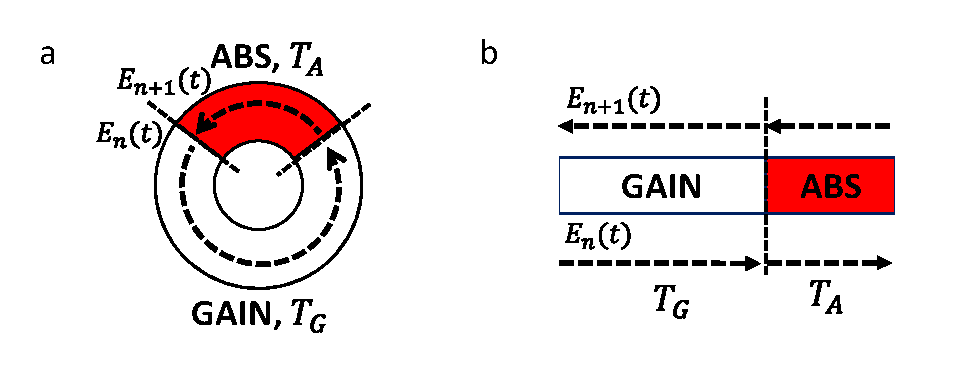
\includegraphics[width=0.7\textwidth]{IMGS/CAVITIES} \label{fig:cavities}\caption{a Ring cavity model. b Fabry-Perot cavity model.}
	\end{figure}
\end{center}

First consider modelocking inside a monolithic Ring cavity as depicted in Fig.~\ref{fig:cavities}a.  Adhereing to Haus's notation, we will denote the envelope profile at the onset of the $n^{th}$ round trip as $E_n(t)$ and with $\tilde E_n(\omega_k) $ the corresponding Fourier component at the angular frequency $\omega_k$.  Notice that here we are refering to quantities related to the slowly varying envelope of the optical field. In order to recover the electric field one needs to apply formula Eq. (\ref{eq:ringansatz-field}) or (\ref{eq:FPansatz-field}), depending on the modelled cavity geometry. 

Upon propagating inside the gain the spectral components of the envelope transform as
\begin{equation}
\label{eq:gainprop}
\tilde E_{nG}(\omega_k) = e^{i\omega_k T_G}e^{G(\omega_k)}E_n(\omega_k), 
\end{equation}
where the first term on the left hand side induces a phase shift due to the delay time $T_G$ and the second term is the frequency dependent gain. Upon passing through the absorber the so modified pulse exhibits further deformation 
\begin{equation}
\label{eq:gainprop}
\tilde E_{n+1}(\omega_k) = \tilde E_{nA}(\omega_k) = e^{i\omega_k T_A}e^{-L(\omega_k)}\tilde E_{nG}(\omega_k) =e^{i\omega_k T_A}e^{-L(\omega_k)} e^{i\omega_k T_G}e^{G(\omega_k)}\tilde E_n(\omega_k). 
\end{equation}
where one must be very careful to 


\section{Some notes/thoughts on the paper}
\subsection{}
	It is important to realize that what matters is the gain recovery time ABOVE THRESHOLD and not to the steady state value w0 of the inversion. This will have a large impact on the mode locking, since for a fixed T1 parameter, the gain recovery time will be shorter if the threshold is LOWER and longer if the threshold is HIGHER. So for ideal results one might want to bias the cavity only slightly above threshold.
\subsection{}
	Note however, that the above argument might not be exactly true. One needs to also consider the losses upon propagating inside the absorber! Assuming perfectly inverted absorber of length $L_a$, without distributed losses, then the condition in Eq. (\ref{eq:threshold-inversion}) becomes
	\begin{align}
	\label{eq:threshold-inversion2}
	&\sigma_{\omega}^{g}N_g\Delta_0^{\text{th}}L_g = aL_g+ \sigma_{\omega}^a N_a L_a, \nonumber \\
	& \Leftrightarrow \nonumber \\
	&\Delta_0^{\text{th}} = \frac{a}{\sigma_{\omega}^{g}N_g} + \frac{\sigma_{\omega}^{a}N_a L_a}{\sigma_{\omega}^{g}N_g L_g}, \nonumber \\
	& \Leftrightarrow \nonumber \\
	&\Delta_0^{\text{th}} = \frac{a}{\sigma_{\omega}^{g}N_g} +  \frac{G_a}{G_g},
	\end{align}
	where subscript/superscript indices $g$/$a$ denote the respective quantities of the gain/absorber section and $G_j = \sigma_{\omega}^{j}N_j L_j$. From Eq. (\ref{eq:threshold-inversion2}), we immediately see that 
	if $G_a>G_g$ then $\Delta_0^{th} > 0$, and no lasing will start whatsoever. 
\subsection{}
	It seems that the mode locking mechanism is very sensitive to the dephasing time $T_{2a}$ of the absorber precisely of that reason! When you DECREASE the pure dephasing time by $T_{2a}\rightarrow T_{2a}/2$, then the absorption cross section $\sigma_\omega^{a} \rightarrow \sigma_\omega^{a}/2$ which LOWERS the threshold $\Delta_{0}^{th}$ due to Eq. (\ref{eq:threshold-inversion2}) and thus broadens the pulse. I expect that the parameter $p$ will thus play a vital role in the dynamics. IDEALLY always keep $p \approx 1$!  
\subsection{}
	Actually we can straight-forwardly derive an expression for the gain recovery time. Assume that the pulse has just passed the atom at time $t=t_0$ and perturbed the system to inversion $\Delta_0(t_0)$. Then the recovery of the gain obeys the simple ODE
	\begin{equation}
	\dot\Delta_0(t) = -\frac{\Delta_0(t) -\Delta_0^{eq}}{T_1},
	\end{equation}    
	which has the solution 
	\begin{eqnarray}
	\Delta_0(t) = \big(\Delta_0(t_0) -\Delta_0^{eq}\big)e^{-\frac{t-t_0}{T_1}}+\Delta_0^{eq}.
	\end{eqnarray}
	Now substituting $\Delta_0^{eq} = p\Delta_0^{(th)}$ and requiring that at $t=t_1$ the gain has recovered to the threshold value $\Delta_0^{th}$ we obtain an equation for the gain recovery time $\Delta T = t_1-t_0$ 
	\begin{equation}
	\Delta_{0}^{th} = \big(\Delta_0(t_0) - p\Delta_0^{th}\big)e^{-\frac{\Delta T}{T_1}}+p\Delta_0^{th}.
	\end{equation}
	with the gain recovery $\Delta T $ given by
	\begin{equation}
	\Delta T = T_1 \ln\frac{p\Delta_0^{th}-\Delta_0(t_0)}{\Delta_0^{th}(p-1)}.
	\end{equation}
	From which we can see that if $p=1$ the gain recovery time will be infinite, which is long enough for mode locking. Naturally this is not acceptable since this would mean that no lasing will be able to start whatsoever and thus the nominator of the fraction will also be small. Therefore what we are seeking to optimize is to maximize the ratio $[p\Delta_0^{th}-\Delta_0(t_0)]/[\Delta_0^{th}(p-1)]$ as a function of $p$. Now we need to see how does the maximal saturation $\Delta_0(t_0)$ depend on the system parameters.
\subsection{}
To investigate the dependence of the maximal saturation $\Delta_0(t_0)$ onto the different parameters we will address the equation
\begin{equation}
\label{eq:inversion3}
\dot\Delta_0(t) = -\frac{\mu^2}{\hbar^2}T_{2} |E|^2\Delta_0(t) -\frac{\Delta_0-\Delta_0^{eq}}{T_1}.
\end{equation}
Assuming instantaneous response of the inversion to the applied field, the population inversion will reach it's minimum as a function of time, at a point where $\dot\Delta_0 = 0$. This readily gives us the solution
\begin{equation}
\label{eq:saturation}
\Delta_0(t_0) = p\Delta_0^{th}\times \frac{1}{\kappa^2T_1T_2|E|^2+1},
\end{equation} 
where $\kappa = \mu/\hbar$ is the coupling parameter. First of all, we notice that $\Delta_0(t_0) >0$ for all $p$. This means that for a fixed pump parameter $p$, the maximum value of the gain recovery is $\Delta T= T_1\times\ln p/(p-1)$. Which can be arbitrarily large for $p\to 1$. There is more to it, as the saturation will not necessarily be 0 but larger. This will depend on the coupling strength $\kappa$, the saturation intensity of the gain medium $I_{sat}\propto 1/T_1T_2$ and the amplitude of the field envelope $|E|$.

Following Haus's solution \cite{haus2000mode}, we know that successful passive mode locking with a fast saturable absorber would produce a hyperbolic secant pulse satisfying the following relations
\begin{align}
E(t) &= E_0 \sech(t/\tau) , \\
\frac{1}{\tau^2} &= {\gamma E_0^2\Omega_g^2}{2g} , \\
l-g &= \frac{g}{\Omega_g^2\tau^2}.
\end{align}

\bibliography{bib_resources.bib}
\end{document}

